\documentclass[10pt]{article}
\usepackage[cm]{fullpage}
\usepackage[utf8]{inputenc}
\usepackage{amsmath}
\usepackage{amsfonts}
\usepackage{comment}
\usepackage{graphicx}
\usepackage{float}

\usepackage{color}
\newcommand\fix[1]{\textcolor{red}{#1}}


\title{How Many Topics to Model?}
\author{Shane Deiley, Mark Heimann, Adrian McLeod}
\date{May 2015}

\begin{document}

\maketitle

\section{Introduction}
With the increasing prevalence of textual data, the desire to discover underlying structure and meaning of this textual data has grown as well.  Spanning various fields, one such text mining technique, \textit{topic modeling}, has applications in bio-informatics, computer vision, music, social science, and more.

The goal of topic modeling is to discover an underlying representation of text documents through the creation of topics. The process begins with data, typically a series of text documents, and ends with a corresponding series of topics, represented by a collection of words that share an underlying relationship with their appearances in the various documents.  As a result, topics can be extremely variable.  For example, a topic analysis on Shakespeare’s plays might output a collection such as: king, sword, feast, death, blood, poison.  The topic may be representing words frequently used together, words of similar meaning, or words of similar context in different stories.

As the necessity for this approach to textual data grows, so the field grows with it.  However, as more topic models are developed, the superiority of one method versus another is not clear.  There is a need, in particular, for a more robust comparison of various topic models qualitatively.  Furthermore, there are various applications of generated topics yet unexplored, including the use of topics in classification settings.  In this paper, we compare the topic quality of two premier topic modeling methods: Latent Dirichlet Allocation (LDA) and Non-negative Matrix Factorization (NMF).  We then use the topics achieved as a label space for classification. 

\section{Text As Data}
In the context of text mining, it may be unintuitive to think about text as a matrix.  However, a term-document matrix is simple to construct, representing various documents as a matrix, where each column is a document and each row is a term from the collective documents' dictionaries of words (see Figure \ref{td-fig}).  The corresponding entry in the term-document matrix is the number of occurrences of that term in the respective document.

\begin{figure}[H]
\centering
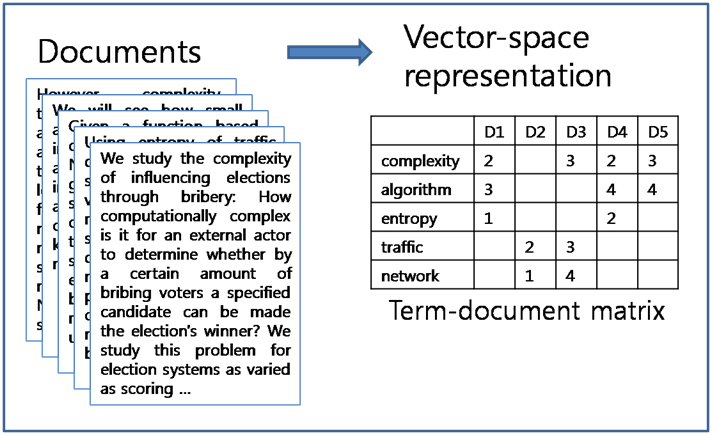
\includegraphics[width=0.6\textwidth, keepaspectratio]{nmf_cluster1-2}
\caption{Transformation of Documents to Data Matrices \cite{td-matrix-pic}}
\label{td-fig}
\end{figure}

\section{Topic Models}

    Topic models, formally, are statistical models that are a class of Bayesian latent variable models.  However, topics can also be viewed as clusters of words with an associated weight for each corresponding document.  Given this interpretation, comparing a formal topic model, such as LDA, with an algorithm that can be interpreted as a topic model \cite{plsa-nmf}, such as NMF, would give us insight as to the performance of these two very different approaches to topic modeling.
    
\subsection{Latent Dirichlet Allocation}

Latent Dirichlet allocation (LDA) \cite{lda} is a complex probabilistic model.  LDA can be thought of as an extension of Probabilistic Latent Semantic Analysis (PLSA).  By placing Dirichlet prior distributions on both the topics and words, a posterior categorical distribution is derived in the presence of the term-document matrix.  This is equivalent to modeling the symmetric form of PLSA with Dirichlet priors and deriving the posterior distribution.

\begin{equation}
\label{LDA}
\Pr(W,Z,\theta,\varphi;\alpha,\beta) = \prod\limits_{i=1}^{K} \Pr(\varphi_i;\beta) \prod\limits_{j=1}^{M} \Pr(\theta_j;\alpha) \prod\limits_{t=1}^{N} \Pr(Z_{j,t}\mid\theta_j)\Pr(W_{j,t}\mid\varphi_{Z_{j,t}})
\end{equation}

Here $W$ is the set of words, $Z$ is the set of topics, $\theta$ is the distribution of topics in each document, and $\varphi$ is the distribution of words for a given topic. We notice the product of each of these distributions in the first two terms; in these terms, $\alpha$ and $\beta$ are the parameters for the Dirichlet prior over $\theta$ and $\varphi$ respectively.  In these products, $K$ is the number of topics, which is determined beforehand.  Further, $M$ is the number of documents with $N_t$ being the number of words in a document $t$. This model can be expressed in plate notation (described in more detail in \cite{plate}), as shown in Figure \ref{lda-fig}.

\begin{figure}[H]
\centering
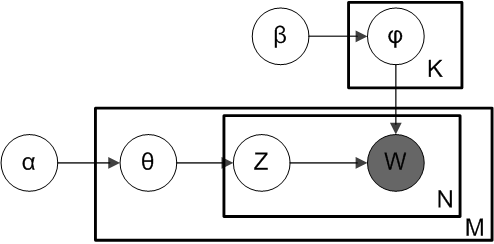
\includegraphics[width=0.4\textwidth, keepaspectratio]{Smoothed_LDA}
\caption{Graphical Model for LDA: Plate Notation \cite{LDA-pic}}
\label{lda-fig}
\end{figure}

Described in words, the first product series is the product of all Dirichlet prior distributions placed on the words for each topic.  This can be thought of as the total probability of words being in any given collection (i.e. of words being in a topic).  The second product series is the product of all of the Dirichlet prior distributions placed on topics per document.  The result is the total probability of documents having intrinsic topic collections.  Finally, we multiply by the distributions of the topics and words given our distribution of topics with respect to the documents and distribution of words with respect to the topics, respectively.

\subsection{Non-negative Matrix Factorization}

Non-negative matrix factorization (NMF) is a matrix decomposition process that reveals intrinsic structure in data.  In the general form, you have an $N \times M$ matrix $V$ and the goal is to decompose it into an $N \times K$ basis matrix $W$ and a $K \times M$ coefficient matrix $H$ such that when multiplied, their product is approximately equal to $V$.

\begin{figure}[H]
\centering
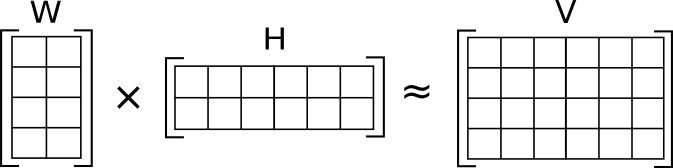
\includegraphics[width=0.65\textwidth, keepaspectratio]{NMF-2}
\caption{Non-negative Matrix Factorization Decomposition \cite{nmf-pic}}
\label{nmf-fig}
\end{figure}

The interesting aspect of this data-reduction method is how the chosen $K$ components of each decomposed matrix interact with the original dimensionality of the data.  Depending on the type and structure of the original data, the $K$ columns of the basis matrix can be thought of as a low-rank representation of the data, or the $K$ rows of the coefficient matrix can be thought of as the weights on the compact basis vectors that reproduce the original data.

The key to this reduction process is the iterative method performed as an approximation of the optimal solution to the objective function.  The following is a standard objective function for NMF (although it is not the only possible or “best” objective function in every situation):

\begin{equation}
\label{NMF-eqn}
\min_{W\ge0,H\ge0} \|V-WH\|_{F}^{2}
\end{equation}

Unfortunately, this objective function is not convex on all the constraints as formulated, meaning the optimal solution must be approximated.  This can be done with multiple optimization techniques that are not crucial to understanding NMF.

Since the text(s) are modeled by an implicitly non-negative term-document (or document-term) matrix, NMF is an applicable method for topic modeling.  As discussed earlier, the result of the decomposition is expected to be $K$ summaries of the original data in the basis matrix.  Each of these vectors will still be of the same length as the dictionary of words (at least in the case of decomposing a term-document matrix), so taking the columns of the basis matrix as they are does generalize well to the real desired topics.  However, after deciding the desired number of words in each topic, it is easy to find the highest counts in each column.  The words with the highest counts in each column are naturally viewed as a topic.  NMF also enables analysis of how important each topic is to each original document.  These weights are found in the coefficient matrix.  The $(k,m)$ entry of the coefficient matrix is the weight of the $k^{th}$ topic to the $m^{th}$ document.  These weights can be interpreted as probabilities by normalizing the sum of the columns of the coefficient matrix to one.

\section{Results}
Using the numpy programming package, we implemented LDA and NMF in order to perform topic modeling on the classic 20 Newsgroups data set \cite{newsgroups}.  After preprocessing the data (removing stop words, stemming, etc.), topic analysis was performed with each method.  For NMF, we could also use a tf-idf re-weighting of the term-document matrix \cite{tf-idf}.  One of our goals was to find a good number of topics to extract from our data. 

\subsection{NMF}
Apart from qualitatively observing the topics sensibility, we attempted to compare our models quantitatively as well.  With a quantitative benchmark of topic quality, we could identify preferable topic counts enabling a more effective label space for our classifier.  A natural measure for this comparison is the model evidence, $P(D|M)$, as it is an intuitive measure of quality to think of the probability of a summary giving the original description.  This is fairly straightforward for LDA, a probabilistic model.  However, for NMF, it was not clear it had a probabilistic interpretation under the objective function presented.  In an attempt to uncover something like model evidence, we thought about the weights in the coefficient matrix.  Since a linear combination of the basis vectors -- i.e. topics -- approximates the original data in NMF, the weights placed on each particular topic are of interest.  The coefficient matrix, a $K x M$ matrix, is comprised of M columns of weights that would approximately reproduce the original M documents.  If each column were scaled so that the sum were one, each entry could be interpreted as a probability.  In this case, we would have $P(T_t|D_j)$, the probability of getting topic $t$ given document $j$.  We further reasoned that we would have $P(W_i|T_t)$, the probability of word $i$ being in topic $t$.  This value would be the $(i,t)^{th}$ entry of the coefficient matrix, provided that the columns are normalized so that they sum to one.  However, with insufficient capabilities of finding $P(D)$ or $P(T)$, we were unsuccessful in finding a valid way to calculate $P(D|M)$ for NMF topics.

\subsection{LDA}
With LDA, we tried two approaches of measuring topic quality quantitatively.  We randomly split our data into training and test sets, where 80\% of the data was used for training and 20\% for testing.  We fit LDA on only the training data.  LDA allows for inference of topic distributions on unseen documents, so for each document in our test as well as training data, we inferred its distribution over the topics we learned.  

The first approach is to calculate the perplexity of our model on the test data to measure how well our probability predicts the test data; the lower the perplexity, the better the model.  

The second approach, proposed in \cite{lda}, is to train a machine learning classifier to predict document category using each document's distribution over topics as features.  Originally, the motivation was to perform classification in a lower dimensional space.  We thought, however, that the results of the classification task might indicate how optimal our number of topics was.  With too few topics, we could have too few features to fit a good classifier, but with too many topics, we might end up overfitting.  Thus, we expected that test error should be a convex function of the number of topics.  

We tested both approaches on "cryptography" and "baseball" articles from the 20 newsgroups dataset.  We performed LDA, varying the number of topics from 3 to 30 by increments of 3.  When fitting LDA, we made 3 passes over the data, as we found that more passes did not seem to give us consistently better results.  For each number of topics, we calculated a lower bound on the log of the perplexity, which we plot in Figure \ref{perplexity}.  We also trained a linear SVM to classify the documents' categories as one or the other based on their distributions over topics, and we plot the test error in Figure \ref{test-error}.

\begin{figure}[H]
\centering
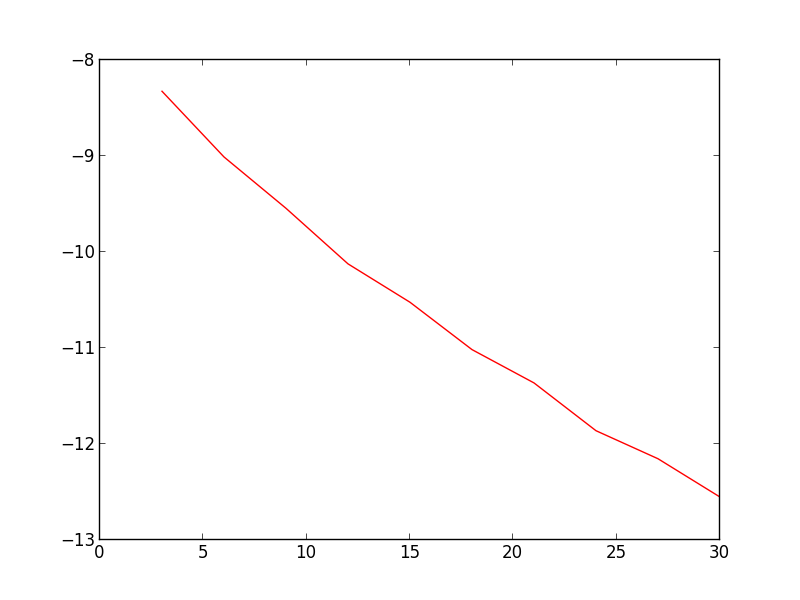
\includegraphics[width=0.6\textwidth, keepaspectratio]{lda-logPerplexity}
\caption{Lower bound on log of perplexity as a function of number of topics}
\label{perplexity}
\end{figure}

\begin{figure}[H]
\centering
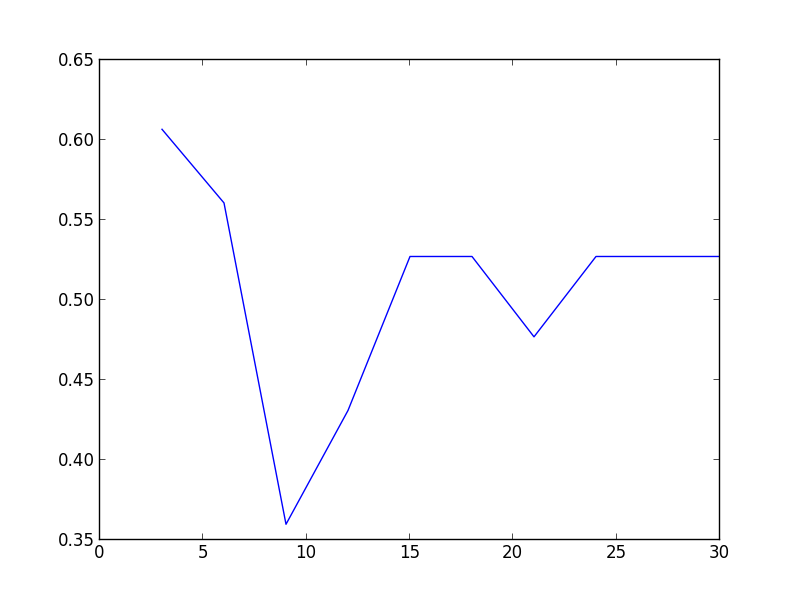
\includegraphics[width=0.6\textwidth, keepaspectratio]{lda-testError}
\caption{Test error as a function of number of topics}
\label{test-error}
\end{figure}

Indeed, up to some noise, we do find that the test error decreases up 9 topics and increases until it levels off (up to some noise) after that.  Unfortunately, our classifier does not do very well.  Indeed, since we are trying to classify documents into 1 of 2 classes, a random classifier should still achieve 50\% accuracy.  Below 6 or above 15 topics, our classifier fails to outperform a random classifier, and even at its best it still has 35\% error.  Thus, it is hard to use these results to infer meaningful conclusions of any kind.  

Also strangely, our perplexity is monotonically decreasing as a function of the number of topics, implying that we never extract enough topics from the data.  Given that we only consider two classes of newsgroups that themselves are not seriously wide-ranging in their scope, this seems unlikely.  A qualitative inspection of some of the topics reveals that with large numbers of topics, individual topics still have recognizable themes (e.g. about technology or baseball), but within each theme (technology or baseball) it is hard to pinpoint a meaningful difference between the topics.  Thus, we would be likely to conclude that with (say) 30 topics, we have extracted too many topics from the data, though the perplexity doesn't show it.  
\section{Discussion and Conclusion}
Perhaps the largest challenge in this project, and what ended up limiting us the most, was actually handling the data.  For a long time, our LDA topics didn't even make sense at all because we failed to adequately pre-process the data, so our data contained clutter such as meaningless symbols, variants of the same word (like "activate", "activation", and "activating"), and so on.  We achieved better results with better pre-processing, but it is possible that we still failed to feed our data to the algorithms in the best form.  Additionally, using more data might help as well.  We ended up having several hundred to low thousands of documents in the reduced two-category dataset on which we performed our LDA experiments.  That may not have been enough to learn a good classifier, particularly with few features.  

The NMF approach, if we could have made it work, seemed promising.  NMF is not a probabilistic model, which is why it would have required more fancy footwork to determine the ideal number of topics to model with it. Nonetheless, NMF ran quickly and produced good results in our initial experiments, so we were excited by it.  LDA took longer to run, but allowed us to try several interesting things like calculate perplexity or infer a document's distribution over topics.  Perhaps our initial results could provoke further work with larger, better-preprocessed data. 

\bibliographystyle{ieeetr}
\bibliography{bib515}

\end{document}
